\chapter{Experimental Results}



\section{Experimental Setup}

This section describes the environment, the data, the models, and the evaluation protocol used throughout the experiments of this chapter. Every result reported in Sections 5.2--5.5 was produced with the pipeline and metrics fixed here, so that the base models, the clustering diagnostics, the dispatchers, and the mixture-of-experts models are directly comparable.

\subsection{Hardware and Software}

All models were trained and evaluated on a single NVIDIA DGX Spark workstation, equipped with a GB10 Grace Blackwell processor with 128 GB of unified memory and a CUDA-capable GPU (CUDA 13.0). Training used PyTorch 2.12 in Python 3.12. Two numerical settings are worth stating because they affect the numbers reported below: \emph{matmuls} run with bfloat16 automatic mixed precision and TF32 enabled, while the loss and all reported metrics are accumulated in single precision (float32). The training tables are stored as compact \texttt{int16} feature indices resident in GPU memory, which is what allows the full dataset to be sampled on-device with \texttt{torch.randint} + gather rather than through a CPU data loader.

\subsection{Dataset and Teacher}

The dataset consists of \textbf{150,815,697 chess positions} stored as 429 memory-mapped \texttt{.npz} slices. Positions are sampled from Lichess human games, a small tactical collection, and high-level bot games, retaining the natural phase distribution of human play (mostly middlegame, fewer openings and endgames). Each position is labeled with a full win/draw/loss distribution from the side-to-move perspective, $\hat{p} = (p_W, p_D, p_L)$, produced by the Leela Chess Zero (Lc0) teacher (network \texttt{791556.pb.gz}) with a single depth-1 MCTS search. We train on the full WDL distribution rather than its scalar summary, which is why the primary loss is soft cross-entropy (Section 5.1.5).

Each FEN is encoded into a sparse binary feature vector of dimension $d_{\text{in}} = 844$ per perspective, split into 716 piece-square features and 128 tactical features (pieces under attack / attacking the king). Two such vectors are produced per position --- one for the side to move and one for the opponent --- giving the dual-POV representation used by the accumulator layer (Chapter 4).

\subsection{Data Splits}

The dataset is partitioned with a stratified per-slice random split: exactly 1\% of each slice is held out as the test set (seed 0), leaving the remaining 99\% for training. This keeps the same phase mix on both sides and prevents any single slice from leaking positions into the test set. The resulting test set contains \textbf{1,507,940 positions}; every test metric reported in this chapter is computed on this fixed set, and no test position participates in clustering, dispatcher training, or expert fine-tuning.

The clustering and dispatcher experiments operate on a representative \textbf{1,000,000-position subsample} of the training split (the same subsample reused across all representations), while the sample-gradient caches used for gradient-based routing are computed on up to 2,000,000 positions. Only summary statistics and projection coordinates are persisted from the clustering stage, never the full cluster assignments.

\subsection{Models and Baselines}

The base models define the reference point against which every MoE variant is judged. They are listed in Table 5.1, together with their parameter counts. The five NNUE models are dual-POV two-hidden architectures of increasing width; the linear, single-hidden FFNN, and dual-hidden FFNN models are dense baselines over the concatenated \texttt{[STM || opp]} features that isolate the contribution of the NNUE inductive bias. One further baseline --- a capacity-matched dense single head with $H{=}512$ (to compare against a $B{=}4,\ H{=}256$ MoE at equal parameter count) --- is planned but not yet trained; it will be added to Table 5.1 when available.

\begin{table}[H]
\centering
\caption{Base models and their test cross-entropy on the fixed 1.5M-position test set.}
\small
\begin{tabular}{lllll}
\toprule
Model & Architecture & $W$ / $H$ & Parameters & Test CE \\
\midrule
Linear & concat \texttt{[STM‖opp]} $\to$ 3 & --- & 5,067 & 0.766 \\
FFNN H64 & single hidden & 64 & 108,291 & 0.669 \\
FFNN H128 & single hidden & 128 & 216,579 & 0.654 \\
FFNN H256 & single hidden & 256 & 433,155 & 0.643 \\
FFNN2 H64 & dual hidden & 64 & 112,451 & 0.656 \\
FFNN2 H128 & dual hidden & 128 & 233,091 & 0.645 \\
FFNN2 H256 & dual hidden & 256 & 498,947 & 0.632 \\
NNUE W32 H64 & dual-POV two-hidden & 32 / 64 & 31,395 & 0.656 \\
NNUE W64 H128 & dual-POV two-hidden & 64 / 128 & 70,979 & 0.672 \\
NNUE W128 H128 & dual-POV two-hidden & 128 / 128 & 141,443 & 0.639 \\
NNUE W128 H256 & dual-POV two-hidden (reference) & 128 / 256 & 174,723 & 0.632 \\
NNUE W256 H512 & dual-POV two-hidden & 256 / 512 & 480,515 & 0.629 \\
\bottomrule
\end{tabular}
\end{table}

The reference model \texttt{W128 H256} is the checkpoint whose head is replaced by expert heads in the MoE experiments, and whose gradients define the routing signal.


The Mixture-of-Experts models evaluated in Section 5.5 share the frozen L1 accumulator of the reference base model and add $K$ expert heads plus a dispatcher. Four routing families are compared: fixed piece-count routing, L1-activation clustering, sample-gradient clustering, and end-to-end soft/sparse gating, each at $K \in \{2,4,8,16\}$ where applicable, alongside an oracle upper bound that assigns each position to the expert with lowest loss, and a random-routing control that isolates the contribution of routing from raw capacity.

\subsection{Training Protocol}

All models are trained with the Adam optimizer at a learning rate of $10^{-2}$ linearly decayed to $10^{-3}$ over 100 epochs. Each epoch consists of 512 batches of 10,000 positions drawn uniformly at random from the training set (5.12M positions per epoch), with the loss accumulated in float32 under bfloat16 AMP. The base models and the dense baselines share this protocol, which makes the parameter-count sweep in Table 5.1 a fair comparison of architecture rather than of training budget. Expert heads in the MoE experiments are fine-tuned from the reference base model, with a minimum of $7\times10^6$ routed samples per expert for the $H{=}256$ heads so that no expert underfits; the preliminary runs in Section 5.5 explicitly report when this budget was not met.

\subsection{Evaluation Metrics}

Accuracy is measured on the held-out test set with four complementary metrics:

\begin{itemize}
  \item \textbf{Cross-entropy (CE)} --- the soft cross-entropy between the model's WDL distribution and the Lc0 teacher distribution, the primary loss and accuracy metric.
  \item \textbf{Mean Absolute Error (MAE)} --- $|v(s) - \hat{v}(s)|$ where $v(s) = p_W - p_L$ is the scalar expected-reward summary of the predicted
\end{itemize}

distribution; MAE is the quantity the search actually consumes.
\begin{itemize}
  \item \textbf{Mean Squared Error (MSE)} and **coefficient of determination ($R^2$)** --- the squared-error analogue and the fraction of target variance explained, reported to characterise the residual distribution of the scalar value.
  \item \textbf{Throughput (NPS)} --- positions evaluated per second, measured both during training and at inference, as the efficiency proxy relevant to deployment.
\end{itemize}



Routing quality (for the dispatchers and the MoE models) is reported with Top-1/Top-2 classification accuracy, macro/weighted F1, and the Adjusted Rand Index (ARI) and Normalized Mutual Information (NMI) against the clustering pseudo-labels. End-to-end playing strength (Elo / ACPL) and on-device search throughput are out of scope for this chapter and are deferred to the deployment evaluation, as they require the full engine integration described in Chapter 4.

\subsection{Experiment Pipeline Overview}

The full battery follows a fixed four-stage pipeline, each stage exporting structured numerical tables and diagnostic plots: (i) \textbf{clustering} of three position representations --- raw board features (1688-d), L1 activations (256-d), and sample-wise head gradients (48-d) --- with mini-batch $k$-means at $k \in \{2,4,8,16\}$, DBSCAN, and a handcrafted piece-count baseline; (ii) **dispatcher
training\textbf{ to map L1 activations (or the board) to bucket IDs, spanning parameter-free cosine-centroid routers, linear/MLP heads, and decision-tree/XGBoost baselines; (iii) }base-model training\textbf{ as in Sections 5.1.4--5.1.5; and (iv) }MoE assembly and fine-tuning** of expert heads per partition. Each stage's results and plots are reported in Sections 5.2 through 5.5.


\section{Clustering}

\subsection{Clustering Algorithm}

The clustering is run on subsamples of the training split rather than on the full corpus of roughly 150 million positions. Exploratory experiments use one million positions drawn from the seed-0 training split (the subsample cached for the base model, with the held-out test positions excluded), and the final partitions are fitted on two million positions. In all cases the sample gradients are computed with respect to the head parameters of the trained base model ($W=128$, $H=256$), L2-normalised so that each vector lies on the unit hypersphere, and the clustering therefore operates on directions rather than magnitudes.

Three candidate representations are clustered in parallel, each evaluated for a range of cluster counts $B$. The first is the raw board encoding, the side-to-move-ordered concatenation of the two 844-dimensional binary views, giving a 1688-dimensional vector. The second is the L1 activation space, the concatenation of the two 128-dimensional accumulator vectors after the side-to-move reorder, giving a 256-dimensional vector. The third is the proposed signal, the sample gradients. Because the flattened head gradient is very high-dimensional, it is projected to a 48-dimensional space through a fixed random (Gaussian) projection before clustering. The board and L1 representations serve as the activation-based references, while the gradients constitute the signal under test.

The primary algorithm is Mini-Batch K-Means with $k$-means++ initialisation, a mini-batch size of $10\,000$, and a fixed random seed, run for $B \in \{2, 4, 8, 16\}$. As a density-based alternative that does not require $B$, DBSCAN is applied with \texttt{min\_samples} fixed at $80$ and $\varepsilon$ selected on a quantile grid to recover a small number of clusters (at most eight). Because the nearest-neighbour density estimates in the native widths are not usable, the board and L1 representations are clustered in a 48-dimensional PCA of the data, whereas the gradient representation is clustered in its native 48-dimensional space. A handcrafted reference partition of eight bins is obtained by bucketing on the scalar piece count, mirroring the conventional NNUE bucketing. The final gradient-based partitions used for the mixture-of-experts are fitted on two million positions for $B \in \{2, 4, 8\}$.

\subsection{Clustering Metrics}

The quality of each partition is assessed with the diagnostics introduced in Section 3.5.5: the silhouette score, which measures how well each point fits its own cluster relative to the nearest other cluster; the within-cluster inertia, which measures compactness; and the pairwise cosine distance between cluster centroids, reported both as a mean and as a minimum, which serves as a proxy for the diversity of the learning signals captured by the buckets. Cluster balance is monitored through the size distribution of the buckets, since a bucket that is too small cannot support stable expert fine-tuning.

In addition, the agreement between partitions is quantified with the adjusted Rand index (ARI) and the normalised mutual information (NMI), both of which measure how well two assignments coincide while correcting for chance. These are used to compare the activation-based and gradient-based partitions with one another and with the piece-count reference. Finally, the stability of the gradient partition is assessed by refitting the clustering on a larger sample and checking that the silhouette and the centroid geometry are preserved as the number of samples increases.

\subsection{Clustering Results}

Table 5.2 reports the mini-batch K-Means diagnostics across the three representations and the piece-count reference. Two findings stand out. First, the gradient-based partitions are markedly better separated than the activation-based ones: for $B=2$ the two gradient centroids are nearly antipodal, with a cosine distance of $1.94$ (a cosine similarity of $-0.94$), and even at $B=16$ the mean cosine distance remains above $1.0$. In contrast, the board and L1 centroids remain close to one another at every value of $B$, with cosine distances well below $0.3$. Second, the gradient partitions achieve the highest silhouette scores of any learned representation at every value of $B$, whereas the L1 silhouette collapses to near zero, and eventually negative, as $B$ grows.

\begin{table}[H]
\centering
\caption{Mini-Batch K-Means clustering diagnostics for the three representations and the piece-count reference, on one million training positions. Silhouette is estimated on a $10\,000$-point subsample; the share columns give the smallest and largest bucket as a fraction of the sample.}
\resizebox{\textwidth}{!}{
  \begin{tabular}{lllllll}
  \toprule
  Representation & $B$ & Silhouette & Cosine dist. (mean) & Cosine dist. (min) & Min. share & Max. share \\
  \midrule
  board & 2 & 0.110 & 0.235 & 0.235 & 0.313 & 0.687 \\
  board & 4 & 0.073 & 0.221 & 0.120 & 0.074 & 0.431 \\
  board & 8 & 0.040 & 0.257 & 0.043 & 0.062 & 0.285 \\
  board & 16 & 0.016 & 0.288 & 0.061 & 0.017 & 0.159 \\
  L1 & 2 & 0.153 & 0.174 & 0.174 & 0.275 & 0.725 \\
  L1 & 4 & 0.109 & 0.208 & 0.115 & 0.104 & 0.541 \\
  L1 & 8 & 0.003 & 0.203 & 0.069 & 0.044 & 0.249 \\
  L1 & 16 & -0.007 & 0.244 & 0.057 & 0.015 & 0.173 \\
  gradients & 2 & 0.250 & 1.938 & 1.938 & 0.441 & 0.559 \\
  gradients & 4 & 0.196 & 1.229 & 0.607 & 0.151 & 0.361 \\
  gradients & 8 & 0.191 & 1.126 & 0.367 & 0.086 & 0.182 \\
  gradients & 16 & 0.134 & 1.049 & 0.123 & 0.034 & 0.131 \\
  piece count & 8 & 0.606 & 0.000 & 0.000 & 0.069 & 0.187 \\
  \bottomrule
  \end{tabular}
}
\end{table}


The piece-count reference attains the highest silhouette score ($0.61$), but this is an artefact of its one-dimensional nature: contiguous, well-separated bins along a single scalar are trivial to recover. Its centroid cosine distance is identically zero, since all bucket means are positive one-dimensional numbers that point in the same direction. The piece-count partition therefore looks compact by silhouette but conveys nothing about the learning signal, and it should not be read as a well-formed candidate for expert specialisation.

The density-based alternative is summarised in Table 5.3. Since the three representations are clustered in different spaces --- the board and L1 encodings in a 48-dimensional PCA of the data and the gradients in the native 48 dimensions --- the three rows are reported per-representation and should not be compared directly. DBSCAN recovers very few clusters from each representation --- three from the board encoding, two from the L1 activations, and five from the gradients --- and it flags a very large fraction of the fit sample as noise: $39.6\%$ for the board encoding, $57.2\%$ for the L1 activations, and $75.2\%$ for the gradients. The recovered clusters are heavily imbalanced, each dominated by a single large core with one or more small satellites, and their silhouette scores, while superficially higher than those of K-Means on the board and L1 data, reflect that dominant core rather than a meaningful multimodal structure. This is consistent with the expectation set out in Section 3.5.3 that density-based clustering is unreliable in a high-dimensional gradient space, and it motivates the use of a fixed $B$ for the mixture-of-experts.

\begin{table}[H]
\centering
\caption{DBSCAN results, fitted on a $100\,000$-point subsample with \texttt{min\_samples}$=80$ and $\varepsilon$ selected on a quantile grid. The board and L1 runs are fit in a 48-dimensional PCA of the data, the gradient run in the native 48 dimensions, so the rows are not directly comparable across representations. Bucket sizes are the cluster shares of the full one-million-position assignment; the noise column gives the fraction of the $100\,000$-point fit flagged as noise.}
\small
\begin{tabular}{lllll}
\toprule
Representation & Clusters & Bucket sizes & Noise (fit subset) & Silhouette \\
\midrule
board & 3 & 78.2\% / 10.5\% / 11.3\% & 39.6\% & 0.172 \\
L1 & 2 & 85.6\% / 14.4\% & 57.2\% & 0.217 \\
gradients & 5 & 21.1\% / 23.1\% / 7.8\% / 40.2\% / 7.7\% & 75.2\% & 0.152 \\
\bottomrule
\end{tabular}
\end{table}


Table 5.4 reports the agreement between the partitions at $B=8$. The board and L1 partitions agree only moderately with each other (NMI $0.24$) and agree weakly with the piece-count reference, suggesting that even activation-based partitions capture structure beyond the game phase. The gradient partition, by contrast, is nearly orthogonal to every other partition: its agreement with the board and L1 assignments is at the level of chance (ARI $0.06$--$0.08$), and its agreement with the piece-count bucketing is essentially zero (ARI $0.04$, NMI $0.09$). This is precisely the behaviour the method is designed to induce: clustering the learning signal recovers a partition that does not simply reproduce the board geometry, the internal representation, or the conventional game-phase bucketing.

\begin{table}[H]
\centering
\caption{Agreement (adjusted Rand index and normalised mutual information) between partitions at $B=8$, computed on one million positions. Higher values indicate closer agreement; the chance baseline is $0$.}
\small
\begin{tabular}{lll}
\toprule
Pair & ARI & NMI \\
\midrule
board vs. L1 & 0.124 & 0.236 \\
board vs. gradients & 0.057 & 0.063 \\
L1 vs. gradients & 0.078 & 0.150 \\
board vs. piece count & 0.189 & 0.303 \\
L1 vs. piece count & 0.147 & 0.290 \\
gradients vs. piece count & 0.042 & 0.088 \\
\bottomrule
\end{tabular}
\end{table}


The final gradient-based clustering, fitted on two million positions for $B \in \{2, 4, 8\}$, reproduces the structure observed on one million positions. The silhouette scores are $0.250$, $0.215$, and $0.179$ for $B=2$, $4$, and $8$ respectively, within $0.02$ of the one-million-position estimates ($0.250$, $0.196$, and $0.191$), and the centroid geometry is preserved, though less tightly at $B=4$: the mean off-diagonal centroid cosine is $-0.938$, $-0.307$, and $-0.128$, against $-0.938$, $-0.229$, and $-0.126$ on the smaller sample --- the $B=2$ and $B=8$ centroids are essentially unchanged, while the $B=4$ centroids drift from $-0.229$ to $-0.307$. The buckets remain well balanced at each value of $B$, ranging from $55.8\%/44.2\%$ at $B=2$ to between $10.8\%$ and $16.0\%$ at $B=8$. The partition is therefore stable with respect to the sample size. As $B$ grows the centroids spread out and their mean pairwise similarity approaches zero: at $B=2$ they are nearly antipodal, while at $B=8$ the pairwise centroid cosines range from strongly negative (near $-0.95$) to moderately aligned (near $+0.72$), consistent with a partition that tiles a single dense gradient manifold rather than isolating well-separated modes.


\begin{figure}[H]
\centering
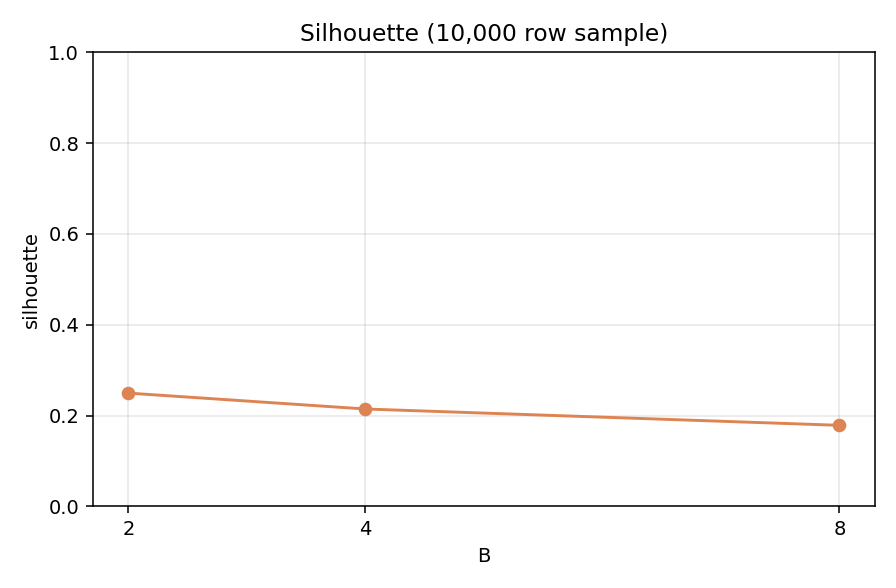
\includegraphics[width=0.60\textwidth]{RESULTS/clustering/plots/previous_gradient_2m/silhouette.png}
\end{figure}



The qualitative evidence supports the quantitative picture. Projections of the gradient space onto the first principal components, and the corresponding t-SNE and UMAP embeddings, show a single connected cloud along which the clusters form contiguous regions, consistent with the low silhouette values and the gradual loss of centroid separation as $B$ increases. In contrast, the L1 and board projections show clusters that are poorly separated and strongly overlapping, mirroring their near-zero cosine distances. The PCA projection of the gradient-based $B=2$ partition in particular shows the two clusters lying on opposite sides of the origin, in line with the antipodal centroids reported above.


\begin{figure}[H]
\centering
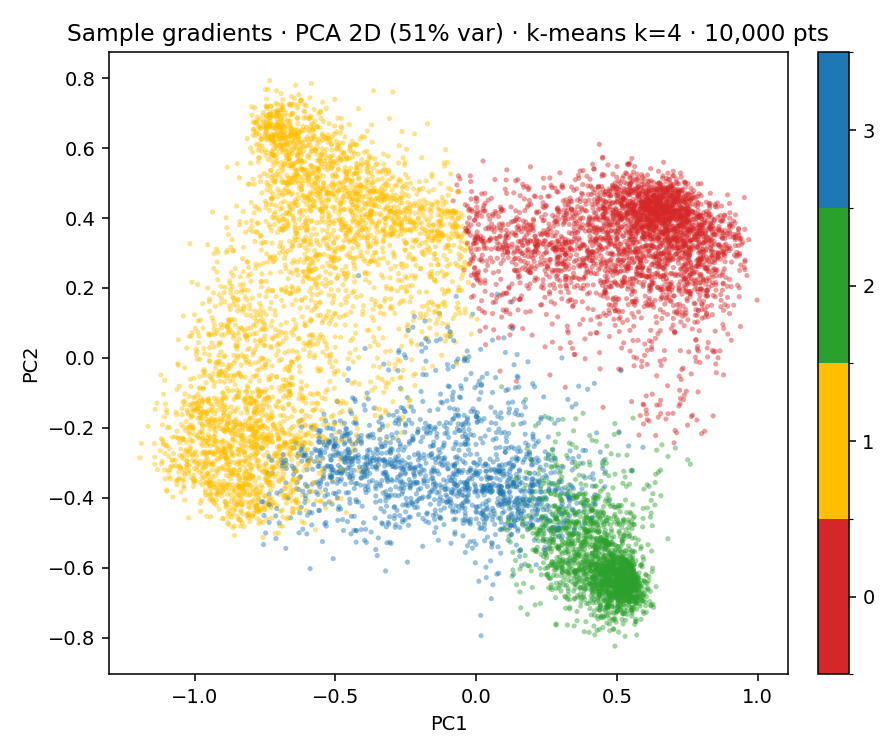
\includegraphics[width=0.60\textwidth]{RESULTS/clustering/plots/pca_2d_gradients.png}
\end{figure}




\begin{figure}[H]
\centering
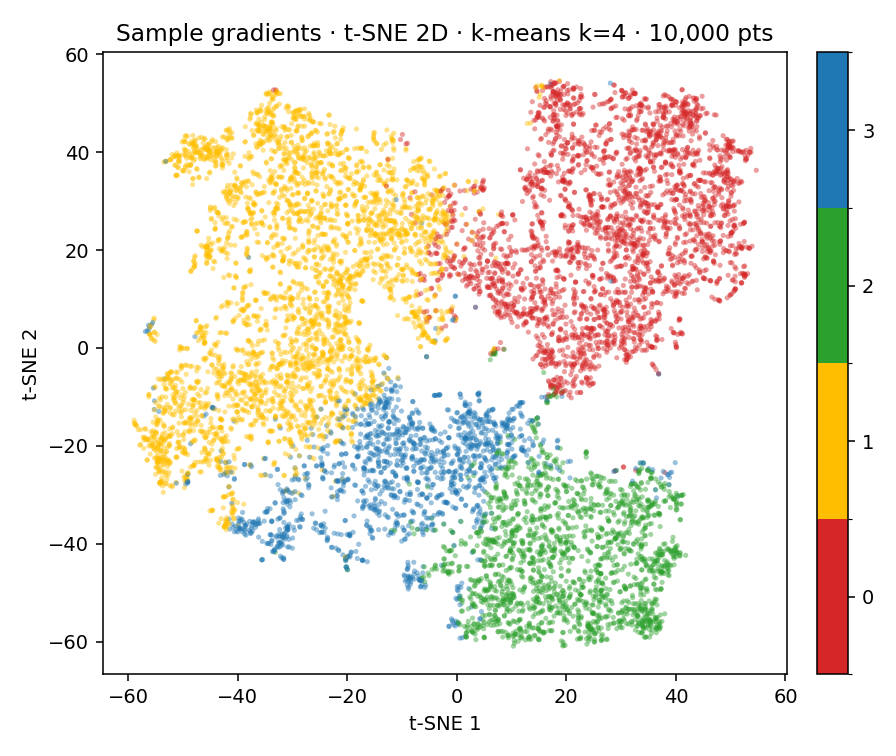
\includegraphics[width=0.60\textwidth]{RESULTS/clustering/plots/tsne_2d_gradients.png}
\end{figure}



Taken together, the results indicate that the gradient-based partition is the most promising candidate for expert specialisation. The antipodal centroids at $B=2$ confirm that the two buckets correspond to opposite directions in head-parameter space --- positions whose gradients pull the head in contrary ways --- which is exactly the kind of diversity the method seeks. The near-zero agreement with the piece-count and activation-based partitions further suggests that these buckets do not correspond to coarse game-phase or geometric categories, but to a genuinely different structure grounded in the learning dynamics. The implication for the mixture-of-experts is that the gradient partition should induce expert task vectors that are more distinct from one another than those produced by any activation-based bucketing, a hypothesis examined in Section 5.5.


\section{Dispatcher}

\subsection{Dispatcher Model}

The dispatcher is a lightweight classifier that maps a position to a bucket index. Its input is the concatenated L1 activation vector, the side-to-move-ordered pair of two $128$-dimensional accumulator views ($256$ dimensions), computed once by the frozen base model and cached for the entire dataset. The primary dispatcher is a single linear layer that produces $B$ logits from the $2W$-dimensional input, with $2W \times B + B$ parameters ($2056$ parameters for $B = 8$) and the softmax used during training is discarded at inference, where the predicted bucket is simply the argmax of the logits. Three alternatives are evaluated to test whether additional capacity is warranted: a single-hidden MLP with $h \in \{32, 64, 128\}$ hidden units, a decision tree (max-depth $12$), and \emph{XGBoost} ($50$ trees of depth $6$). A parameter-free centroid router is evaluated as an additional reference: each position is assigned to the bucket whose $k$-means centroid is nearest in cosine similarity, using either the $1688$-dimensional board-state centroids or the $256$-dimensional L1 centroids.

The distinction between the offline clustering and the dispatcher is central to the method. The partition is defined in sample-gradient space, which is unavailable at inference time --- computing a gradient would require the teacher evaluation of the position --- so the partition cannot be applied directly to an unseen position. The dispatcher instead predicts the bucket from L1 activations, a feature that is already produced by the incremental accumulator update during the normal forward pass. The centroid routers serve as the geometric upper bound of what the partition allows to be recovered from the representation alone: they reproduce the partition exactly as far as the representation's geometry permits, without any learned non-linearity. The learned dispatcher is trained to approximate the partition with cross-entropy against the $k$-means labels, using Adam with a learning rate of $10^{-2}$ decayed to $10^{-3}$, a batch size of $1024$, eight epochs, and a $90/10$ train/validation split on one million positions. Note that the $k$-means labels are computed on the full one-million-position subsample before the split, so the validation accuracy reported below is transductive rather than a fully independent estimate. Because the L1 activations are cached, each router trains in a few seconds to a minute on a GPU.

\subsection{Dispatcher Metrics}

The dispatcher is scored against the pseudo-ground-truth cluster labels produced by Mini-Batch $k$-Means, using the agreement metrics introduced in Section 3.5.5. Top-1 and top-2 accuracy report how often the correct bucket is the single highest (or among the two highest) predicted logits; the macro-F1 and weighted-F1 scores summarise per-bucket precision and recall, with the weighted variant reflecting the imbalanced bucket sizes; and the adjusted Rand index (ARI) and normalised mutual information (NMI) quantify the agreement between the predicted and reference partitions while correcting for chance. A normalised confusion matrix and per-class precision-recall curves are produced for each router.

Two trivial baselines are reported alongside every learned router. The \emph{chance} baseline predicts uniformly at random, achieving $1/B$; the \emph{dummy} baseline always predicts the majority cluster. Because the buckets are imbalanced, the dummy baseline is the more demanding reference, ranging from $0.727$ at $B=2$ to $0.172$ at $B=16$ for the L1 partitions, and from $0.560$ to $0.134$ for the gradient partitions. The piece-count rule-based router is evaluated separately by its ARI/NMI alignment with the learned partitions, since it defines its own eight buckets rather than predicting an existing partition.

\subsection{Dispatcher Results}

Table 5.5 reports the two parameter-free centroid routers. Both reproduce the Euclidean $k$-means partition well above chance, but the L1 centroids do so markedly better than the board-state centroids: the L1 router attains a top-1 accuracy of $0.979$ at $B=2$, falling only to $0.940$ at $B=16$, while the board router falls from $0.946$ to $0.817$ over the same range. The corresponding ARI values track the same ordering ($0.916 \to 0.892$ for L1 versus $0.791 \to 0.620$ for the board), and the NMI values show the L1 agreement actually \emph{increasing} with $B$ ($0.846 \to 0.884$) while the board agreement peaks near $B=8$ and declines. The L1 partition is therefore recoverable almost entirely through a cosine-nearest-centroid rule, confirming that the activation-based buckets are geometrically well separated, whereas the board-state partition is only partially expressible from its centroid geometry. Because the routers assign points by cosine proximity but are scored against the Euclidean $k$-means labels, these figures are a lower bound on recoverability: scoring against a spherical (cosine) $k$-means, which matches the routing rule, would raise the agreement further.

\begin{table}[H]
\centering
\caption{Parameter-free centroid routers (\texttt{argmin} cosine similarity to the $k$-means centroids), scored against the Euclidean Mini-Batch $k$-Means labels on one million positions. Chance is $1/B$; the majority dummy ranges from $0.727$ ($B=2$) to $0.172$ ($B=16$) for the L1 labels.}
\small
\begin{tabular}{lllll}
\toprule
Representation & $B$ & Top-1 & ARI & NMI \\
\midrule
board & 2 & 0.946 & 0.791 & 0.670 \\
board & 4 & 0.898 & 0.731 & 0.700 \\
board & 8 & 0.875 & 0.701 & 0.763 \\
board & 16 & 0.817 & 0.620 & 0.723 \\
L1 & 2 & 0.979 & 0.916 & 0.846 \\
L1 & 4 & 0.963 & 0.909 & 0.856 \\
L1 & 8 & 0.948 & 0.893 & 0.872 \\
L1 & 16 & 0.940 & 0.892 & 0.884 \\
\bottomrule
\end{tabular}
\end{table}



\begin{figure}[H]
\centering
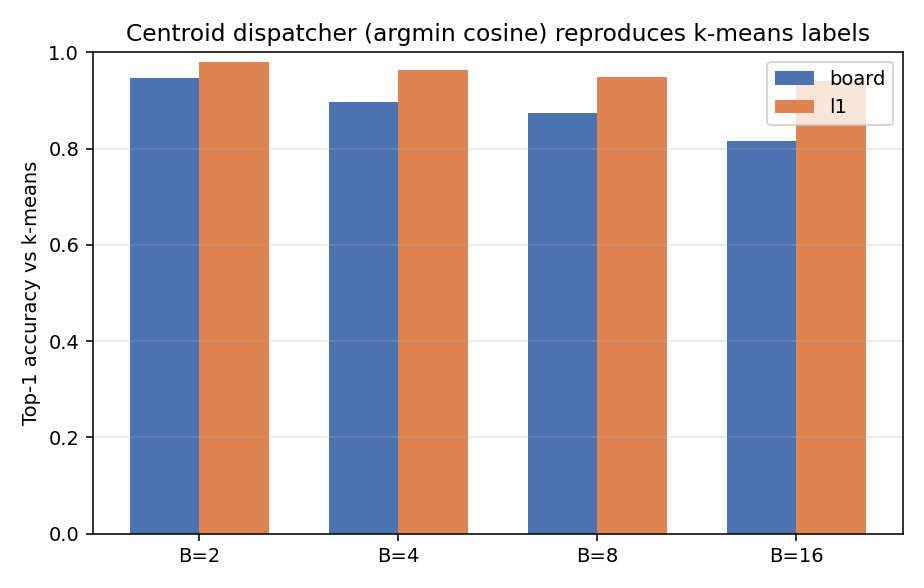
\includegraphics[width=0.60\textwidth]{RESULTS/dispatcher/centroid/plots/accuracy.png}
\end{figure}



Table 5.6 reports the learned routers trained to predict the L1 $k$-means buckets from L1 activations. Recovery of the L1 partition is essentially trivial for the neural routers: the linear dispatcher reaches $0.993$ at $B=2$ and $0.967$ at $B=16$, and the single-hidden MLP is statistically indistinguishable from it ($0.994 \to 0.971$). XGBoost approaches the neural routers ($0.986 \to 0.891$), while the single decision tree is the weakest of the four ($0.959 \to 0.704$), although even it clears the dummy baseline by a wide margin. The ARI values confirm the same ranking, with the linear and MLP routers preserving more than $0.94$ of the partition structure up to $B=16$, XGBoost $0.80$, and the decision tree $0.51$. Since the buckets are imbalanced, the macro-F1 (not shown) sits slightly below the weighted-F1 at every $B$, but the ordering across routers is unchanged.

\begin{table}[H]
\centering
\caption{Learned L1-to-L1 dispatchers on one million positions ($90/10$ split), scored against the L1 Mini-Batch $k$-Means labels. Chance is $1/B$; the majority dummy is $0.727$, $0.542$, $0.248$, and $0.172$ for $B=2,4,8,16$ respectively.}
\small
\begin{tabular}{llll}
\toprule
Router & $B$ & Top-1 & ARI \\
\midrule
linear & 2 & 0.993 & 0.972 \\
linear & 4 & 0.988 & 0.969 \\
linear & 8 & 0.978 & 0.952 \\
linear & 16 & 0.967 & 0.937 \\
MLP ($h{=}64$) & 2 & 0.994 & 0.973 \\
MLP ($h{=}64$) & 4 & 0.990 & 0.975 \\
MLP ($h{=}64$) & 8 & 0.980 & 0.957 \\
MLP ($h{=}64$) & 16 & 0.971 & 0.945 \\
decision tree & 2 & 0.959 & 0.835 \\
decision tree & 4 & 0.906 & 0.788 \\
decision tree & 8 & 0.794 & 0.595 \\
decision tree & 16 & 0.704 & 0.512 \\
XGBoost & 2 & 0.986 & 0.942 \\
XGBoost & 4 & 0.967 & 0.921 \\
XGBoost & 8 & 0.930 & 0.850 \\
XGBoost & 16 & 0.891 & 0.799 \\
\bottomrule
\end{tabular}
\end{table}



\begin{figure}[H]
\centering
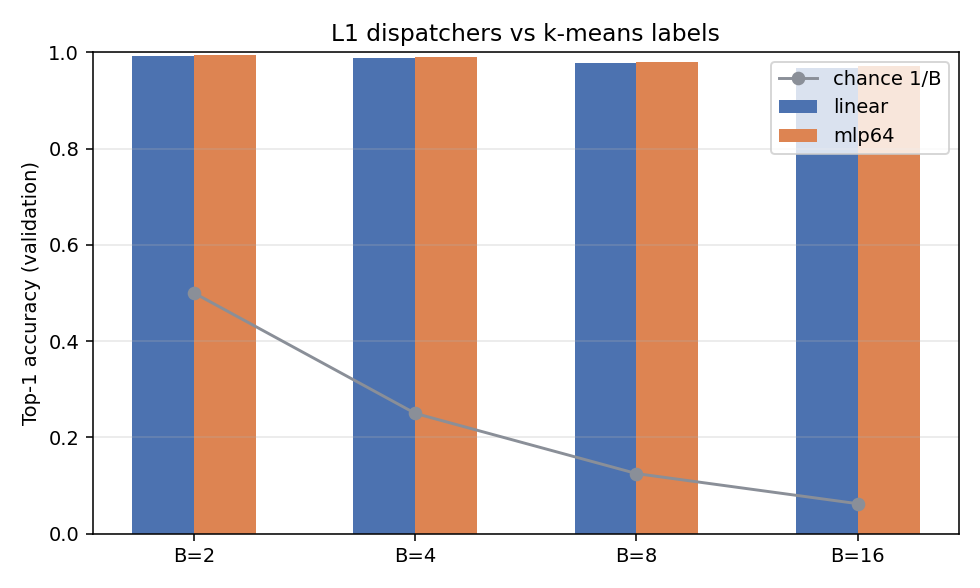
\includegraphics[width=0.60\textwidth]{RESULTS/dispatcher/l1/plots/accuracy.png}
\end{figure}




Varying the hidden width of the MLP router between $32$, $64$, and $128$ units makes essentially no difference on the L1 target: at every value of $B$ the three widths agree within $0.003$ in top-1 accuracy (for instance $0.993$--$0.994$ at $B=2$ and $0.970$--$0.973$ at $B=16$), and the ARI values are likewise indistinguishable. The L1 partition is linearly recoverable to begin with, so additional non-linear capacity has nothing to exploit.

The picture reverses when the routers are trained to predict the \emph{gradient} $k$-means buckets from L1 activations, as shown in Table 5.7. Here recovery is much harder: top-1 accuracy falls from $0.63$--$0.64$ at $B=2$ to $0.47$--$0.49$ at $B=16$, and the ARI remains at or below $0.37$ throughout. The routers do exceed the dummy baseline --- substantially so at the larger values of $B$ (for instance $0.47$--$0.49$ against a dummy of $0.134$ at $B=16$) --- but at $B=2$ the MLP routers barely clear the $0.560$ majority label, and their ARI of $0.07$--$0.08$ indicates agreement only marginally above chance. Hidden width again matters little: the three widths are within $0.01$ of one another at every $B$. A separate linear gradient dispatcher, trained earlier on the two-million-position gradient cache at $B \in \{2,4,8\}$, reaches validation accuracy $0.60$, $0.56$, and $0.48$; it is omitted from Table 5.7 because it is trained on a different subsample than the MLP sweep reported here. This is the central negative result of the dispatcher study: \textbf{L1 activations are a weak proxy for gradient direction}, and no amount of learned non-linearity of the size tested here recovers the gradient partition. The gradient clustering therefore carries routing information that is not present in the activation representation, which is precisely the motivation for gradient-based routing in the first place --- but it also means that the deployable L1 dispatcher cannot faithfully reproduce that partition, a limitation quantified further in Section 5.5.


\begin{table}[H]
\centering
\caption{MLP dispatchers (hidden width $h$) trained to predict the gradient $k$-means buckets from L1 activations, on one million positions ($90/10$ split). Chance is $1/B$; the majority dummy is $0.560$, $0.361$, $0.184$, and $0.134$ for $B=2,4,8,16$ respectively.}
\small
\begin{tabular}{lllll}
\toprule
Target & $h$ & $B$ & Top-1 & ARI \\
\midrule
gradient & 32 & 2 & 0.642 & 0.081 \\
gradient & 64 & 2 & 0.632 & 0.069 \\
gradient & 128 & 2 & 0.642 & 0.081 \\
gradient & 32 & 4 & 0.580 & 0.226 \\
gradient & 64 & 4 & 0.587 & 0.225 \\
gradient & 128 & 4 & 0.588 & 0.228 \\
gradient & 32 & 8 & 0.522 & 0.362 \\
gradient & 64 & 8 & 0.525 & 0.366 \\
gradient & 128 & 8 & 0.530 & 0.369 \\
gradient & 32 & 16 & 0.475 & 0.367 \\
gradient & 64 & 16 & 0.483 & 0.368 \\
gradient & 128 & 16 & 0.490 & 0.369 \\
\bottomrule
\end{tabular}
\end{table}



\begin{figure}[H]
\centering
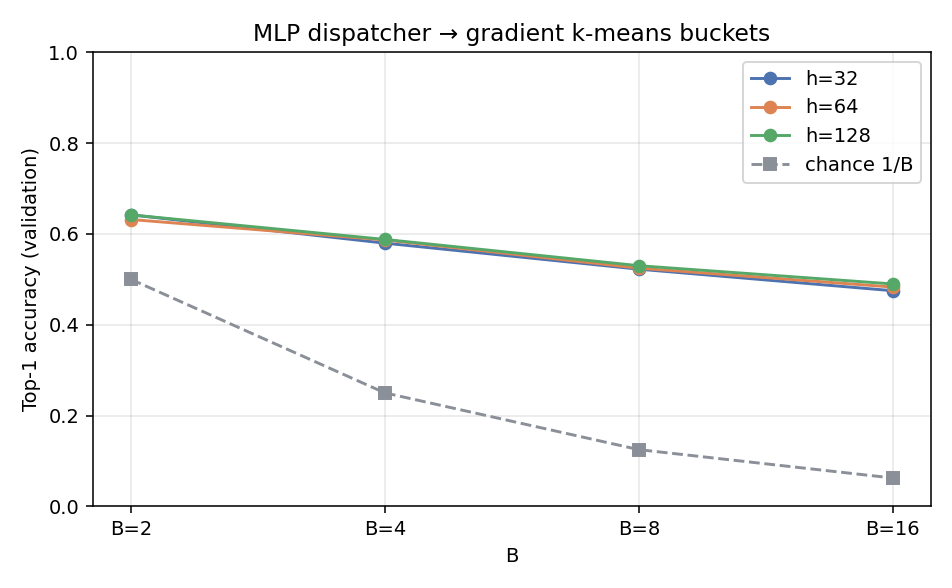
\includegraphics[width=0.60\textwidth]{RESULTS/dispatcher/mlp/plots/accuracy_gradient.png}
\end{figure}




\begin{figure}[H]
\centering
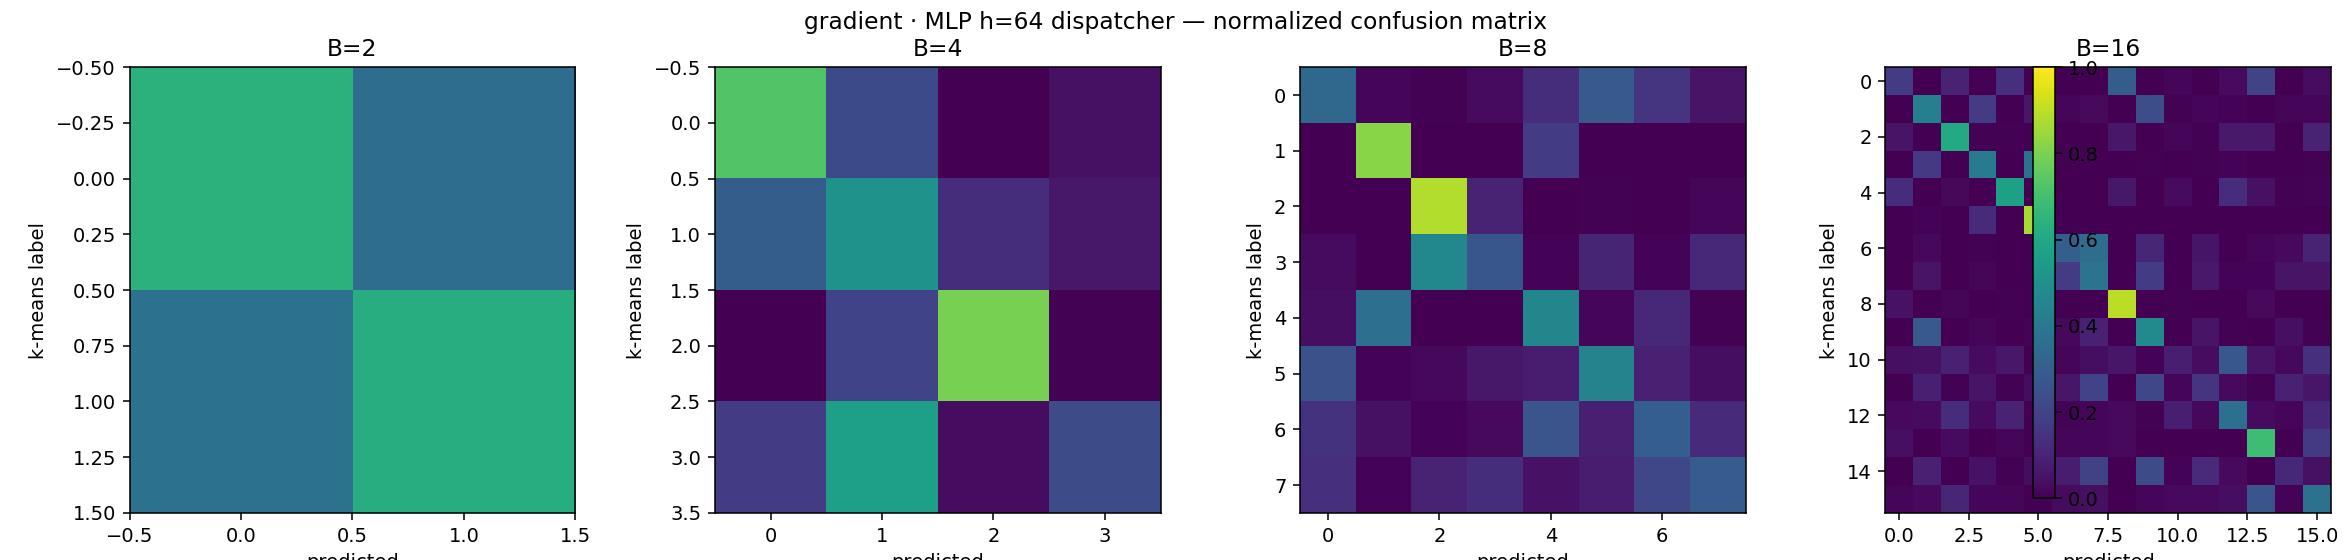
\includegraphics[width=0.60\textwidth]{RESULTS/dispatcher/mlp/plots/confusion_gradient.png}
\end{figure}




The macro-F1 consistently lags the top-1 accuracy by a growing margin as $B$ increases (for instance $0.40$--$0.42$ against $0.47$--$0.49$ at $B=16$), indicating that the smaller buckets are disproportionately misclassified: the majority buckets dominate the top-1 accuracy, while the per-bucket precision and recall are dragged down by the rare buckets. The learned routers are therefore a poor \emph{point} approximation of the gradient partition, although --- as the ARI of $0.37$ at $B=16$ shows --- they retain a coarse, non-trivial signal that exceeds the majority and chance baselines at every value of $B$.

The fixed eight-interval piece-count router is evaluated purely by its alignment with the learned partitions, since it predicts its own bucket definitions. Table 5.8 shows that it aligns weakly with the L1 partitions (ARI $0.11$--$0.17$) and essentially not at all with the gradient partitions (ARI $0.01$--$0.05$). The piece-count buckets themselves are reasonably balanced, with the eight intervals covering between $6.9\%$ and $18.7\%$ of the sample. This mirrors the clustering findings of Section 5.2.3: piece count is a one-dimensional game-phase signal that shares little structure with either activation- or gradient-based buckets, and it cannot serve as a substitute for the learned routing.

\begin{table}[H]
\centering
\caption{Alignment (ARI/NMI) between the fixed eight-bucket piece-count router and the L1 and gradient $k$-means partitions at each $B$, computed on one million positions.}
\small
\begin{tabular}{llll}
\toprule
Target & $B$ & ARI & NMI \\
\midrule
L1 & 2 & 0.108 & 0.254 \\
L1 & 4 & 0.168 & 0.358 \\
L1 & 8 & 0.147 & 0.290 \\
L1 & 16 & 0.126 & 0.314 \\
gradient & 2 & 0.008 & 0.014 \\
gradient & 4 & 0.014 & 0.037 \\
gradient & 8 & 0.042 & 0.088 \\
gradient & 16 & 0.045 & 0.120 \\
\bottomrule
\end{tabular}
\end{table}



\begin{figure}[H]
\centering
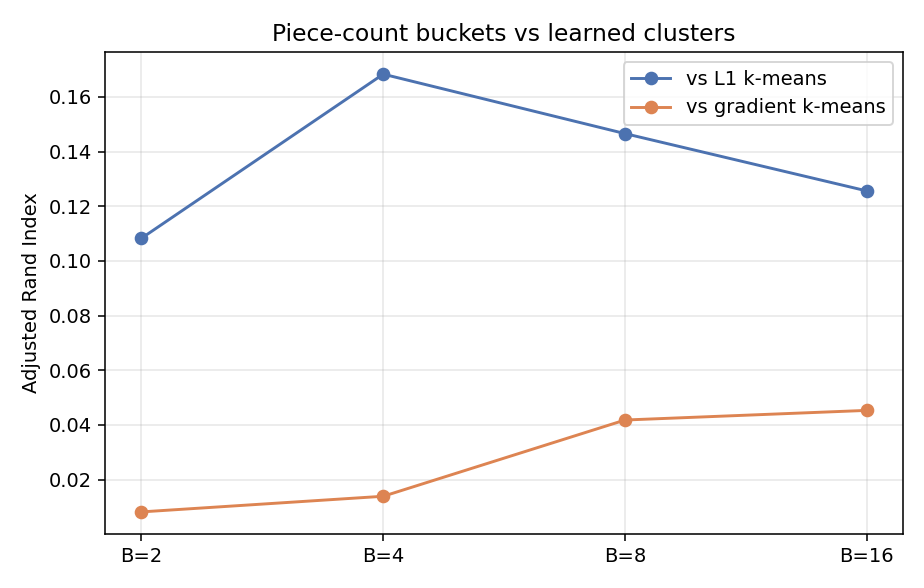
\includegraphics[width=0.60\textwidth]{RESULTS/dispatcher/piececount/plots/alignment.png}
\end{figure}



The computational and memory overhead of the dispatcher is negligible relative to the evaluation function. The linear router holds $2W \times B + B$ parameters --- $2\,056$ for $B=8$ and $4,112$ for $B=16$ --- and the largest MLP variant tested ($h=128$) still holds fewer than $40,000$ parameters, orders of magnitude below the shared L1 accumulator. At inference the dispatcher adds a single matrix-vector product over $B$ outputs followed by an argmax, both inexpensive integer operations that precede the (unchanged) head forward pass; on the target hardware this is bounded by the cost of a $2W \times B$ multiply-accumulate. Training is similarly cheap, completing in seconds per router because the L1 activations are precomputed.


\section{Base Model}

\subsection{Base Model Architecture and Training}

The base model is the dual-POV two-hidden NNUE described in Chapter 4: a sparse binary input of $d_{\text{in}}=844$ features per perspective, a shared accumulator L1 ($844 \to W$) run once for each POV with CReLU clipping to 127, the two $W$-dimensional accumulator vectors concatenated in side-to-move order ($2W$), a second hidden layer L2 ($2W \to H$) with the same CReLU non-linearity, and a linear head ($H \to 3$) producing the side-to-move $(W,D,L)$ logits normalised by softmax. Five widths were trained, $(W,H) \in \{(32,64),(64,128),(128,128),(128,256),(256,512)\}$, spanning 31k to 481k parameters; the $(128,256)$ model is the reference used throughout the MoE experiments, both for its frozen L1 accumulator and as the source of the sample-gradient routing signal.

Training follows the protocol of Section 5.1.5: Adam with a learning rate of $10^{-2}$ linearly decayed to $10^{-3}$ over 100 epochs of 512 batches of 10,000 positions, soft cross-entropy against the Lc0 WDL distribution, accumulated in float32 under bfloat16 AMP on the int16 compact feature tables.

Three dense baselines isolate the contribution of the NNUE inductive bias. All operate on the side-to-move-ordered concatenation of the two raw 844-d views ($2\times844$ features) rather than the shared dual-POV accumulator: a linear head (concat $\to 3$), a single-hidden FFNN (concat $\to H \to 3$), and a dual-hidden FFNN (concat $\to H_1 \to H_2 \to 3$), each with a CReLU on its hidden activations. They match the reference NNUE in depth and roughly in width while removing the shared-accumulator structure, so the gap between them and the NNUE at equal parameter count is a direct measure of the inductive bias.

\subsection{Base Model Metrics}

The base models are scored on the fixed 1.5M-position test set with the metrics of Section 5.1.6. The primary accuracy figure is the soft cross-entropy (Table 5.1); for the dense baselines the full regression suite is also reported --- MAE and MSE on the scalar expected value $v = p_W - p_L$ and the coefficient of determination $R^2$ --- together with the model size and the measured inference throughput (positions per second on the compact dense path). The scaling of test CE with training-set size is evaluated by retraining the $H=64$ and $H=256$ models on progressively larger training subsamples.

\subsection{Base Model Results}

Table 5.9 reports the dense baselines with their full metrics. The linear model (5,067 parameters) reaches CE 0.766 / MAE 0.258 / $R^2$ 0.716; the single-hidden FFNN improves monotonically with width (CE 0.669 $\to$ 0.643, $R^2$ 0.842 $\to$ 0.880 for $H=64\to256$); the dual-hidden FFNN adds a second CReLU layer and recovers most of the remaining gap (CE 0.656 $\to$ 0.632, $R^2$ 0.856 $\to$ 0.893). Crucially, at equal or larger parameter count the flat FFNN still underperforms the NNUE: FFNN H256 (433k parameters, CE 0.643) is worse than the reference NNUE W128 H256 (175k parameters, CE 0.632), and even the dual-hidden FFNN2 H256 (499k parameters, CE 0.632) only \emph{matches} the reference NNUE at nearly three times the parameter count. This is the NNUE inductive bias at work: the shared, POV-reused accumulator and the sparse input give the NNUE strictly better predictive quality per parameter.

\begin{table}[H]
\centering
\caption{Dense baselines (linear, single-hidden FFNN, dual-hidden FFNN) with full regression metrics and inference throughput on the 1.5M-position test set. The reference NNUE W128 H256 (174,723 parameters) attains CE 0.632, beating the dual-hidden FFNN2 H256 at 2.9$\times$ the parameters.}
\resizebox{\textwidth}{!}{
  \begin{tabular}{lllllll}
  \toprule
  Model & Parameters & Test CE & Test MAE & Test MSE & $R^2$ & Infer NPS \\
  \midrule
  Linear & 5,067 & 0.766 & 0.258 & 0.139 & 0.716 & 2.56M \\
  FFNN H64 & 108,291 & 0.669 & 0.172 & 0.077 & 0.842 & 2.69M \\
  FFNN H128 & 216,579 & 0.654 & 0.157 & 0.067 & 0.863 & 2.70M \\
  FFNN H256 & 433,155 & 0.643 & 0.145 & 0.059 & 0.880 & 2.62M \\
  FFNN2 H64 & 112,451 & 0.656 & 0.161 & 0.071 & 0.856 & 2.58M \\
  FFNN2 H128 & 233,091 & 0.645 & 0.149 & 0.062 & 0.873 & 2.65M \\
  FFNN2 H256 & 498,947 & 0.632 & 0.135 & 0.053 & 0.893 & 2.56M \\
  \bottomrule
  \end{tabular}
}
\end{table}


Across the five NNUE widths (Table 5.1), test CE falls to 0.629 at the largest model $(W{=}256,H{=}512)$. The reference $W{=}128,H{=}256$ model --- chosen because its 2M-position gradient cache already exists and its head is the seed of the expert heads in the MoE --- attains CE 0.632 at 174,723 parameters, within 0.003 of the largest model. (The $W{=}64,H{=}128$ point is the sole non-monotonicity of the sweep and is treated as an outlier of the early width grid.)

The scaling of test CE with training-set size, shown for the $H=64$ and $H=256$ models in the figure below, improves steeply at first and then plateaus: the $H=256$ model reaches CE $\approx 0.631$ by roughly 30M positions and then oscillates within $\pm 0.002$ out to 90M; the smaller $H=64$ model levels off near CE $\approx 0.660$ by roughly 70M positions. The reference model was therefore trained deep into the plateau. Critically for Section 5.5, the expert heads in the MoE experiments are fine-tuned on only 2M positions, far to the left of the region where the base architecture even begins to saturate; this data-starvation of the experts, rather than any architectural limitation, is the recurring explanation for the modest MoE results reported below.


\begin{figure}[H]
\centering
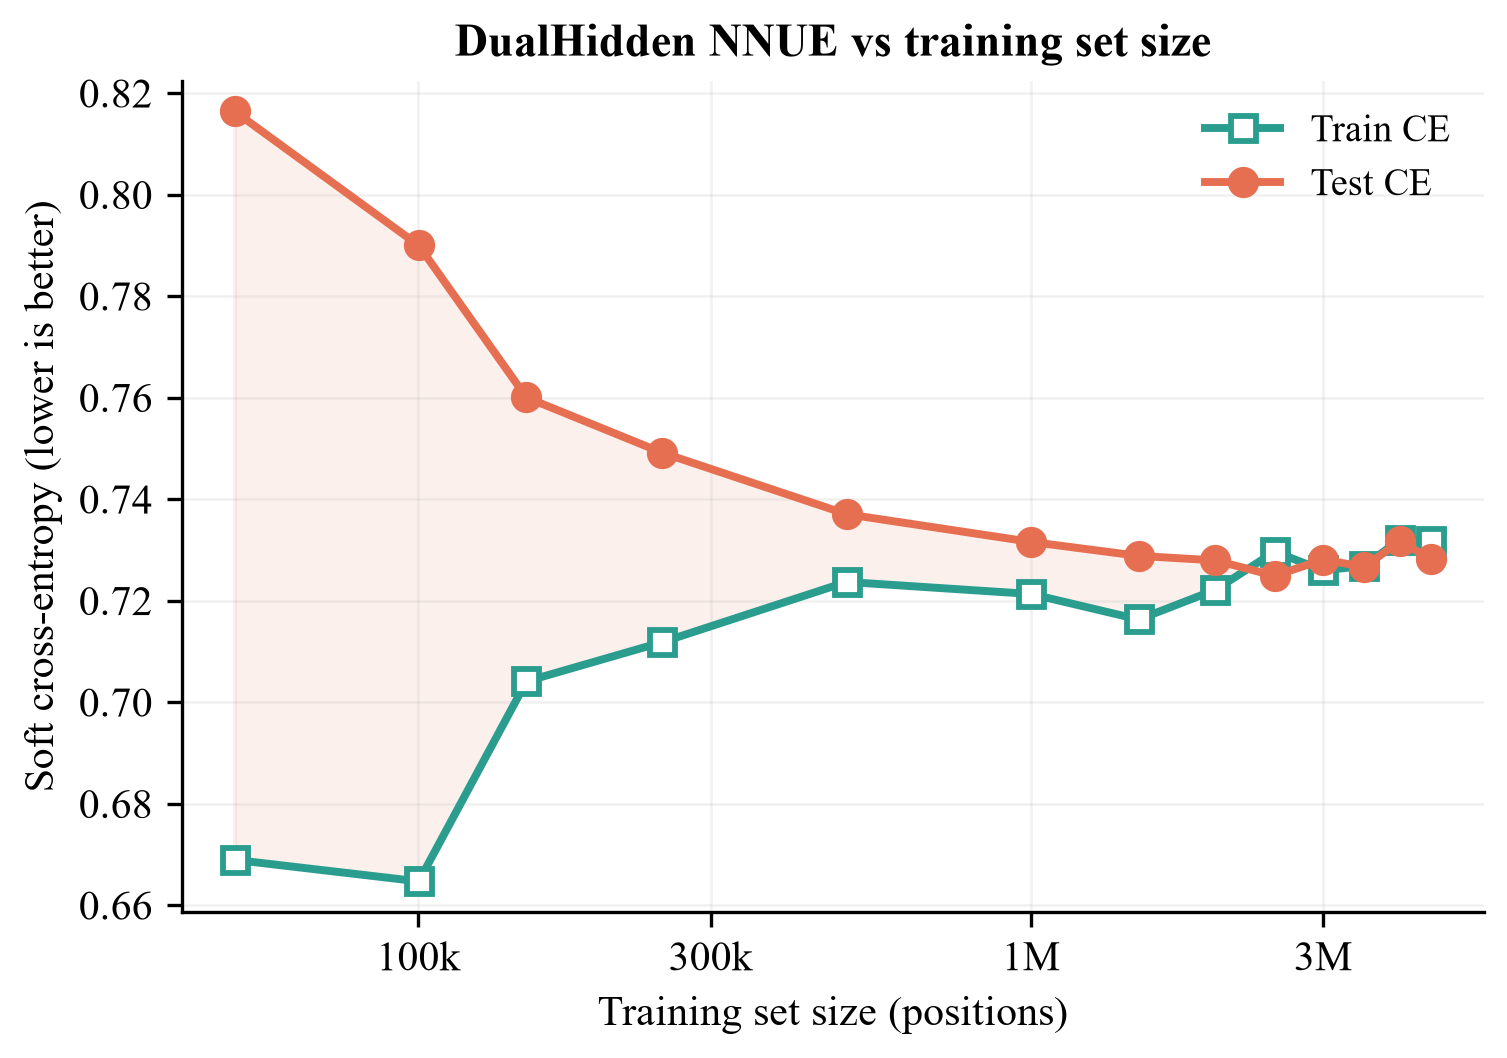
\includegraphics[width=0.60\textwidth]{RESULTS/base/scaling/nnue_ce_vs_train_size.png}
\end{figure}



The reference base model is thus established as W128 H256, with full-test CE 0.632 (Table 5.1) and, on the 50,000-position subsample used for the MoE comparisons of Section 5.5, CE 0.6303 and MAE 0.1326. Every MoE variant in the next section is judged against this model with the same frozen L1 accumulator.


\section{Mixture of Experts}

\subsection{MoE Architecture and Training}

Every MoE variant shares the frozen L1 accumulator of the reference base model (W128 H256) and replaces its single head with $K$ expert (L2, head) blocks, each cloned from the base head and then fine-tuned. At inference a router selects one (hard) or a blend (soft) of the $K$ experts; L1 is never updated, so only the L2/head blocks and the router parameters are trained. The experts are therefore true \emph{specialists} in the sense that their inductive bias is inherited from the base and only the per-bucket behaviour is re-learned.

Four routing families and three controls are compared, each at $K \in \{2,4,8,16\}$ where applicable:

\begin{enumerate}
  \item \textbf{Piece-count} --- fixed eight-interval handcrafted bucketing on the scalar piece count (Section 5.2), with no training; this is the conventional NNUE bucketing baseline.
  \item \textbf{L1-clustered hard MoE} --- mini-batch $k$-means on the 256-d L1 activations, plus an MLP dispatcher ($h{=}64$) mapping L1 $\to$ bucket ID.
  \item \textbf{Gradient-clustered hard MoE} --- mini-batch $k$-means on the 48-d sample head gradients, plus an MLP dispatcher ($h{=}64$) mapping L1 $\to$ gradient bucket ID.
  \item \textbf{End-to-end soft-gated MoE} --- a differentiable top-1/top-2 softmax gate trained jointly with the experts and an auxiliary load-balancing loss.
  \item \textbf{Switch (end-to-end sparse top-1)} --- hard argmax top-1 routing with the load-balancing loss swept over $\alpha \in \{0.001, 0.01, 0.05\}$.
  \item \textbf{Oracle upper bound} --- retroactive $\arg\min_k \mathcal{L}_k$ routing (each position sent to its minimum-loss expert), an unachievable ceiling that uses the target at inference.
  \item \textbf{Random dispatcher control} --- uniform random routing over the same experts, to isolate the contribution of routing from raw capacity.
\end{enumerate}


All experts are fine-tuned on the 2M-position training pack (\texttt{moe\_b4\_2m}), with frozen L1: two epochs per expert for the hard (dispatcher) variants and five epochs of joint training for the soft-gated and Switch variants. This gives $2\times10^6/K$ routed rows per expert --- far below the $7\times10^6$-per-expert budget identified for $H{=}256$ in Section 5.1.5 --- so every expert is trained in a data-starved regime relative to the base model's scaling behaviour (Section 5.4.3). The consequence of this shortfall is visible in every result below.

\subsection{MoE Metrics}

Each MoE is scored on the 50,000-position test subsample used throughout this chapter, against the reference base (CE 0.6303, MAE 0.1326 on this subsample). The primary figures are the soft cross-entropy and the expected-value MAE of the complete MoE; for the hard variants the dispatcher's top-1 accuracy against its pseudo-ground-truth buckets is reported alongside, and for the soft variants the gate entropy and the load-balance variance quantify whether routing actually specialises. Per-bucket expert CE (vs. the base head's CE on the same bucket) measures whether individual experts improve on their own subset. The oracle and random-router evaluations use the exact same expert weights and test set, differing only in how the bucket index is chosen.

\subsection{MoE Results}

Table 5.10 summarises the three hard variants. The headline is uniformly negative: \textbf{no routing variant beats the base.} The piece-count MoE (K=8) is exactly tied with the base (CE 0.6303), and its per-bucket expert CE equals the base CE on every bucket --- piece count carries no specialisation signal. The L1-clustered MoE is trivially recoverable by its dispatcher (top-1 0.996 $\to$ 0.980) yet gains essentially nothing: its CE ranges from 0.6309 (K=2) to 0.6300 (K=16), a -0.0003 edge at best. The gradient-clustered MoE is the most interesting: its dispatcher recovers the gradient partition only weakly (top-1 0.643 $\to$ 0.476, consistent with Section 5.3.3), yet it is the only variant that edges out the base on CE at the larger $K$ (0.6300 at K=8, 0.6301 at K=16). The weak dispatcher is exactly what caps it --- the routing signal is present in the experts but not recoverable from L1.

\begin{table}[H]
\centering
\caption{Dispatcher-routed hard MoE (piece-count, L1-clustered, gradient-clustered) on the 50,000-position test subsample. The reference base attains CE 0.6303 and MAE 0.1326 on this subsample. "Dispatcher Top-1" is the MLP dispatcher's accuracy against its own k-means pseudo-labels (L1 or gradient).}
\small
\begin{tabular}{lllll}
\toprule
Variant & $K$ & Dispatcher Top-1 & MoE CE & MoE MAE \\
\midrule
piece-count & 8 & --- (fixed rule) & 0.6303 & 0.1331 \\
L1-clustered & 2 & 0.996 & 0.6309 & 0.1343 \\
L1-clustered & 4 & 0.992 & 0.6305 & 0.1343 \\
L1-clustered & 8 & 0.986 & 0.6303 & 0.1332 \\
L1-clustered & 16 & 0.980 & 0.6300 & 0.1327 \\
gradient-clustered & 2 & 0.643 & 0.6307 & 0.1338 \\
gradient-clustered & 4 & 0.587 & 0.6306 & 0.1345 \\
gradient-clustered & 8 & 0.534 & 0.6300 & 0.1328 \\
gradient-clustered & 16 & 0.476 & 0.6301 & 0.1330 \\
\bottomrule
\end{tabular}
\end{table}



\begin{figure}[H]
\centering
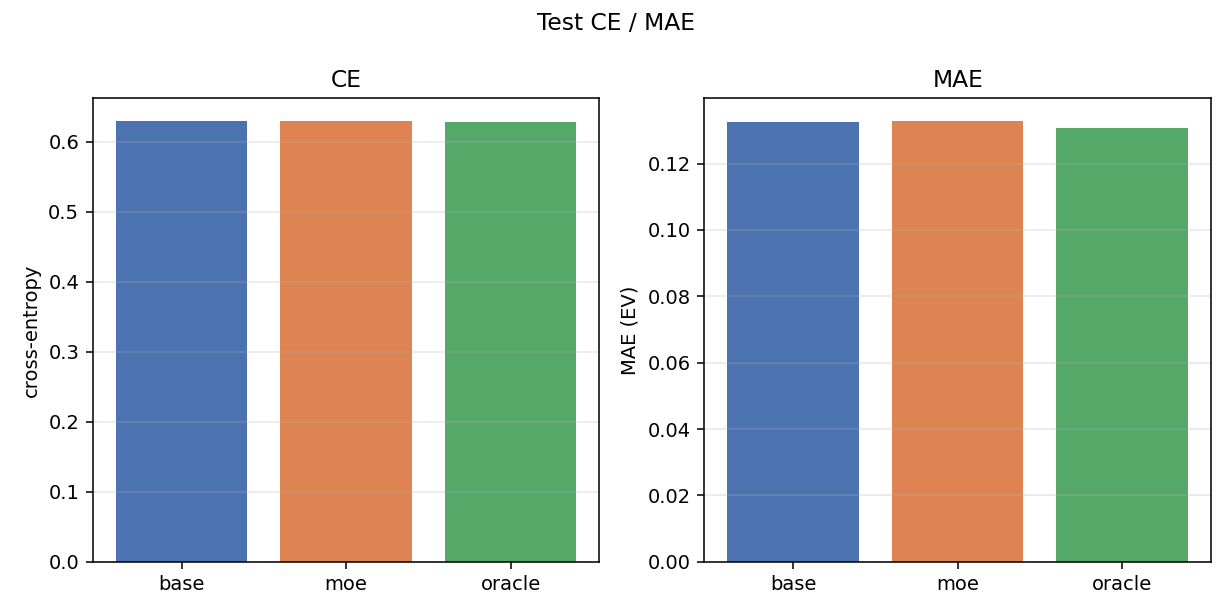
\includegraphics[width=0.60\textwidth]{RESULTS/moe/grad_clustered_k16/plots/moe_vs_base_ce.png}
\end{figure}



Table 5.11 reports the jointly-trained soft gate. It, too, fails to beat the base. The best configuration is top-2 with $K=2$ (CE 0.6304), which is the only run whose MAE improves on the base (0.1324 vs. 0.1326) even as its CE is slightly worse; top-2 beats top-1 at every $K$, and performance degrades monotonically with $K$ because the extra experts only add parameters that underfit the 2M-position budget. The gate entropy sits at $\ln K$ throughout and the load variance is $\approx 0$: the load-balancing loss pins the router near-uniform, so the gate never learns to specialise and the experts remain near-clones of the base head.

\begin{table}[H]
\centering
\caption{End-to-end soft-gated MoE test CE (top-1 and top-2 gating), on the 50,000-position subsample. Base CE 0.6303. Gate entropy $\approx$ ln K and load variance $\approx$ 0 at every setting.}
\small
\begin{tabular}{lllll}
\toprule
Top-k & $K{=}2$ & $K{=}4$ & $K{=}8$ & $K{=}16$ \\
\midrule
top-1 & 0.6307 & 0.6315 & 0.6317 & 0.6323 \\
top-2 & 0.6304 & 0.6306 & 0.6306 & 0.6310 \\
\bottomrule
\end{tabular}
\end{table}


Table 5.12 reports the Switch-style hard top-1 variant across the load-balancing weight $\alpha$. It reproduces the soft-gated top-1 behaviour and adds nothing: the best run is $\alpha{=}0.001$, $K{=}2$ (CE 0.6307), and $\alpha$ barely matters (a given $K$ varies by $\leq 0.0003$ across $\alpha$). The hard argmax gate receives no gradient through the CE path --- only through the load-balancing term --- so it drifts toward uniform and, like the soft gate, never specialises; larger $K$ again only adds underfit parameters.

\begin{table}[H]
\centering
\caption{Switch (end-to-end sparse top-1) test CE vs. load-balancing weight $\alpha$, on the 50,000-position subsample. Base CE 0.6303.}
\small
\begin{tabular}{lllll}
\toprule
$\alpha$ & $K{=}2$ & $K{=}4$ & $K{=}8$ & $K{=}16$ \\
\midrule
0.001 & 0.6307 & 0.6312 & 0.6316 & 0.6326 \\
0.01 & 0.6307 & 0.6312 & 0.6317 & 0.6323 \\
0.05 & 0.6309 & 0.6313 & 0.6319 & 0.6325 \\
\bottomrule
\end{tabular}
\end{table}


The most informative result is the oracle (Table 5.13). Routing each test position to its $\arg\min_k \mathcal{L}_k$ expert reveals large, monotonic headroom: CE falls from 0.6244 (K=2) to 0.6005 (K=16), with MAE reaching 0.088 at K=16 against the base's 0.133. The experts genuinely \emph{can} specialise. Two further facts sharpen this. First, the nearest-gradient-centroid proxy oracle (Section 5.3.3's routing rule) is far weaker --- 0.6280 at K=16 --- so the gradient centroids are \emph{not} the argmin-loss partition: the partition implied by "route to the closest gradient centroid" is a different, much weaker one than "route to the best expert". Second, the realised dispatcher MoE sits at $\approx$0.630, an order of magnitude farther from the oracle than the oracle is from a perfect model. The entire gap is therefore a \emph{routing} gap, not a \emph{capacity} gap: the experts hold the information, but no deployable signal (L1 activations, or even gradient centroids) can recover the assignment.

\begin{table}[H]
\centering
\caption{Oracle upper bound on the gradient-clustered experts, on the 50,000-position subsample. "Dispatcher CE" is the realised MLP-routed MoE; "Nearest-centroid CE" is the cosine/nearest-centroid routing rule of Section 5.3.3; "Oracle CE" is the true $\arg\min_k \mathcal{L}_k$ routing. The oracle uses the target at inference and is an unachievable upper bound.}
\resizebox{\textwidth}{!}{
  \begin{tabular}{llllll}
  \toprule
  $K$ & Base CE & Dispatcher CE & Nearest-centroid CE & Oracle CE & Oracle MAE \\
  \midrule
  2 & 0.6303 & 0.6307 & 0.6320 & 0.6244 & 0.1242 \\
  4 & 0.6303 & 0.6306 & 0.6312 & 0.6160 & 0.1145 \\
  8 & 0.6303 & 0.6300 & 0.6291 & 0.6067 & 0.1006 \\
  16 & 0.6303 & 0.6301 & 0.6280 & 0.6005 & 0.0881 \\
  \bottomrule
  \end{tabular}
}
\end{table}



\begin{figure}[H]
\centering
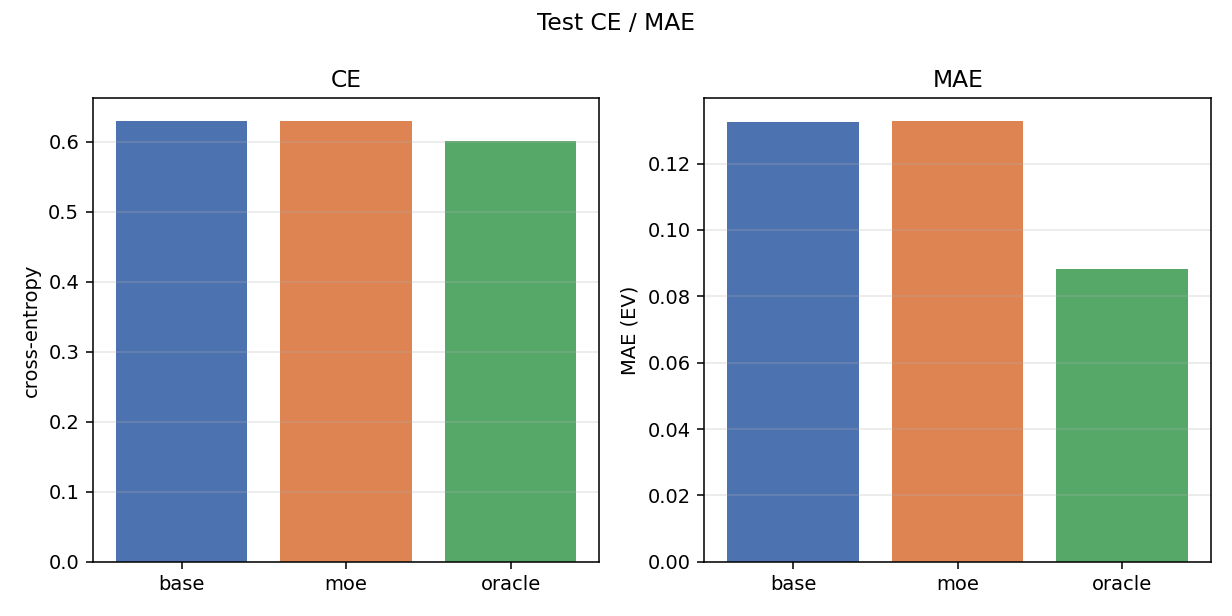
\includegraphics[width=0.60\textwidth]{RESULTS/moe/oracle_k16/plots/moe_vs_base_ce.png}
\end{figure}



Finally, Table 5.14 replaces the trained dispatcher with a uniform random router over the same experts. Random routing is always \emph{worse} than the trained dispatcher and \emph{worse than the base}, and it degrades with $K$ (gradient: 0.6311 $\to$ 0.6398; L1: 0.6317 $\to$ 0.6346). This is the complement of the oracle result: each fine-tuned expert has drifted from the generalist base into a specialist, so a random expert is a poor generalist on out-of-bucket positions. The trained dispatcher's routing is precisely what "buys back" that drift and returns the MoE to $\approx$ base --- confirming that the (small) difference between the MoE and the base is a routing effect, not a capacity effect.

\begin{table}[H]
\centering
\caption{Random dispatcher control (uniform random routing over the same experts), on the 50,000-position subsample. Base CE 0.6303; the trained-dispatcher MoE CE is given in Table 5.10.}
\small
\begin{tabular}{lllll}
\toprule
Variant & $K{=}2$ & $K{=}4$ & $K{=}8$ & $K{=}16$ \\
\midrule
gradient-clustered & 0.6311 & 0.6337 & 0.6429 & 0.6398 \\
L1-clustered & 0.6317 & 0.6327 & 0.6341 & 0.6346 \\
\bottomrule
\end{tabular}
\end{table}


Read together, the three controls tell a coherent story. The oracle shows the experts carry real, monotonic specialisation headroom (0.600 at K=16). The random router shows that, without correct routing, the same experts are worse than the base and degrade with $K$. And the realised dispatchers --- the only deployable routers --- sit essentially on top of the base, because the routing signal they can consume (L1 activations, or even gradient centroids) is too weak to recover the argmin assignment. The mixture-of-experts hypothesis therefore fails not for lack of capacity or specialisation, but for lack of an \emph{inference-time} signal that identifies the right expert; quantifying and, if possible, closing that gap is the central open question carried into the Discussion.


\section{Summary of Experimental Findings}

The empirical results of this chapter can be condensed into six findings.

\begin{enumerate}
  \item \textbf{Clustering.} Sample head gradients are a markedly better-separated and more stable routing representation than board features or L1 activations, and they are nearly orthogonal to the piece-count and activation partitions (Section 5.2.3).
\end{enumerate}


\begin{enumerate}
  \item \textbf{Dispatcher approximation.} L1 activations recover the L1 partition almost perfectly (top-1 $\approx 0.97\text{--}0.99$) but the gradient partition only weakly (top-1 $\approx 0.49\text{--}0.64$, ARI $\leq 0.37$): L1 activations are a poor proxy for gradient direction (Section 5.3.3).
\end{enumerate}


\begin{enumerate}
  \item \textbf{Base model.} The dual-POV two-hidden NNUE is the best architecture per parameter, and its quality saturates only at 30--70M training positions --- far beyond the 2M positions available for expert fine-tuning (Section 5.4.3).
\end{enumerate}


\begin{enumerate}
  \item \textbf{No routing gain.} No MoE variant --- piece-count, L1-clustered, gradient-clustered, soft-gated, or Switch --- beats the reference base on test CE; the best results tie it, and most are slightly worse (Section 5.5.3).
\end{enumerate}


\begin{enumerate}
  \item \textbf{The gap is routing, not capacity.} The oracle upper bound shows large monotonic headroom (CE 0.600 at $K{=}16$), while the random-router control shows the same experts are worse than the base without correct routing. The experts hold the information; the deployable routing signal does not (Section 5.5.3).
\end{enumerate}


\begin{enumerate}
  \item \textbf{Gradient centroids are not the argmin partition.} Even perfect nearest-gradient-centroid routing (CE 0.628 at $K{=}16$) falls far short of the true argmin oracle (0.600), so the clustering objective and the routing objective diverge.
\end{enumerate}


The Discussion will examine in depth: (i) the stability and separability of the gradient partition; (ii) why L1 activations fail to approximate gradient direction and whether an alternative inference-time feature could; (iii) the mismatch between the clustering objective and the argmin-loss routing objective; (iv) the extent to which the $2\times10^6$-position expert budget --- versus the $\sim 30\times10^6$ the base needs to saturate --- is the binding constraint on expert specialisation; and (v) the computational trade-offs of the MoE head relative to a single dense head of equal capacity.